\documentclass[10pt,a4paper]{article}
\usepackage[margin=1.4cm,top=1.1cm,bottom=1.2cm]{geometry}
\usepackage{mathptmx}
\usepackage[T1]{fontenc}
\usepackage{amsmath,amssymb}
\usepackage{microtype}
\usepackage{booktabs}
\usepackage{float}
\usepackage{enumitem}
\usepackage{titlesec}
\usepackage{caption}
\usepackage{xcolor}
\usepackage{tikz}
\usetikzlibrary{positioning}
\usepackage{listings}
\setlist{nosep,leftmargin=1.3em}
\titleformat{\section}{\normalsize\bfseries}{\thesection}{0.6em}{}
\titlespacing*{\section}{0pt}{4pt}{1pt}
\captionsetup{font=small,labelfont=bf,skip=3pt}
\setlength{\parindent}{0pt}
\setlength{\parskip}{2pt}
\pagestyle{empty}

% Marker for content that still has to be filled in by the group.
\newcommand{\todo}[1]{\textcolor{red}{\textbf{[TODO: #1]}}}

% Small R listing style for the condensed code
\lstdefinestyle{rcode}{
  language=R,
  basicstyle=\ttfamily\fontsize{6.1}{7.0}\selectfont,
  commentstyle=\itshape\color{gray},
  keywordstyle=\bfseries,
  showstringspaces=false,
  columns=fullflexible,
  keepspaces=true,
  breaklines=true,
  breakindent=0pt,
  aboveskip=0pt, belowskip=0pt,
  xleftmargin=0pt, framexleftmargin=0pt,
  frame=none
}

\begin{document}

\begin{center}
{\large\bfseries Assignment 2 - Part 2}\\[3pt]
{\small 2AMS11 Survival Analysis for Data Science --- Group Assignment, Part II --- October 2026}\\[1pt]
{\small\textbf{Group 49:} Avram Andrei, Mihaiescu Cristian, Szelestey Adam, Vrincianu Darius, Zeng Qin Tao}
\end{center}
\vspace{-8pt}

\section{Response to Feedback}
\textbf{Feedback received:} ``The only comment I have is that you do not look up the literature after Gemini gave you information about TPE and liver failure. Can you check this for the next assignment?''
\textbf{How it was addressed:} We fact-checked the information from Gemini Pro against the literature. TPE is used in acute liver failure (ALF) either as a ``bridge'' to liver recovery or to maintain stability until a transplant is possible (Chris-Olaiya et al., 2021, p.~906; Larsen et al., 2016). Older age is strongly associated with a higher accumulation and severity of extrahepatic comorbid diseases, such as cardiovascular disease, chronic kidney disease and type 2 diabetes (Jepsen, 2014, pp.~7223--7225). Metabolic comorbidities (obesity, type 2 diabetes, dyslipidemia) are the primary drivers of metabolic problems associated with steatotic liver disease (Huang et al., 2023, pp.~389--391). Patients receiving TPE for ALF are critically ill intensive-care patients whose trajectory is determined within days to weeks by either native hepatocyte recovery or emergency transplant, which makes outpatient hospital readmission an uninformative metric for acute TPE efficacy (Chris-Olaiya et al., 2021, pp.~905--906). This literature justified moving away from a hospital-readmission framework. In Part I we instead define the failure event as transplant-free survival (time to death or liver transplant), observed from the first TPE cycle with right-censoring at 90 days (Larsen et al., 2016, pp.~70--72; Chris-Olaiya et al., 2021, p.~906).
\textbf{Suggestions not adopted:} none; the single suggestion was adopted.

\section{Simulation algorithm}
Our goal is to generate synthetic datasets from the Part~I model and then fit parametric models to the observed values, which helps us answer the following research questions:
\textbf{RQ1.} How accurately (bias, variance, MSE) does the log-logistic model estimate the true $\beta$'s, and how does this change with sample size ($n=200$ vs.\ $500$) and loss to follow-up (5\% vs.\ 10\%)?
\textbf{RQ2.} How biased are the estimates if we (a) fit a Weibull model, which cannot capture the early peak, or (b) leave out the confounder age?

\textbf{Setup.} Fix the true parameters (Table~\ref{tab:par}) and $\gamma=1.1$, $\tau=90$ days, $n\in\{200,500\}$, loss to follow-up $p\in\{5\%,10\%\}$ and $R=2000$ runs. For each $p$, find $c_{\max}$ numerically (\texttt{uniroot}, on $10^6$ simulated patients) such that $P(L<\min(T,\tau))=p$, with $L\sim U(0,c_{\max})$. This is the probability that a patient is lost to follow-up before their event or the 90-day cutoff. Then, for each of the four scenarios $(n,p)$ and each run $r=1,\dots,R$:
\begin{enumerate}[label=(\alph*),itemsep=0pt]
\item \textbf{Generate covariates} $D,A,K,E$ for $n$ patients from the distributions in Table~\ref{tab:par}.
\item \textbf{Generate event times} $T=\lambda\,(U/(1-U))^{1/\gamma}$ with $U\sim U(0,1)$ and $\lambda=\exp(\beta_0+\beta_D D+\beta_E E+\beta_A A+\beta_K K)$ (inverse-CDF method).
\item \textbf{Generate censoring times} $C=\min(\tau,L)$ with $L\sim U(0,c_{\max})$.
\item \textbf{Construct the observed dataset:} $Y=\min(T,C)$ (\texttt{time}) and $\Delta=I\{T\le C\}$ (\texttt{status}).
\item \textbf{Fit the models} with \texttt{survreg}: M1 log-logistic with all covariates (RQ1), M2 Weibull with all covariates (RQ2a), M3 log-logistic without age (RQ2b).
\item \textbf{Store} $\hat\beta$, the scale ($=1/\hat\gamma$ for the log-logistic model) and the standard errors of each fit. Fits that fail or do not converge are skipped and counted.
\item \textbf{Repeat} for all $R=2000$ runs and four scenarios, then compute the performance measures.
\end{enumerate}
In the code, all $n\cdot R$ patients of a scenario are generated at once and split into runs by \texttt{run\_id}.

\begin{table}[H]
\centering\footnotesize
\caption{Covariates, their R names and true effects ($\beta_0=5.8$). $\phi=e^{\beta}$ is the time ratio per unit.}\label{tab:par}
\begin{tabular}{@{}lllrr@{}}
\toprule
Covariate & R name & Distribution & $\beta$ & $\phi$ \\
\midrule
$D$: days from diagnosis to TPE & \texttt{days} & $\mathrm{Gamma}(2,\ \text{scale } 2)$ & $-0.10$ & $0.90$ \\
$A$: age (years) & \texttt{age} & $\mathcal N(45,15^2)$, capped to $[18,85]$ & $-0.02$ & $0.98$ \\
$K$: number of comorbidities & \texttt{nr\_comor} & $\mathrm{Poisson}$, mean $e^{-2.75+0.05A}$ & $-0.25$ & $0.78$ \\
$E$: damage outside the liver & \texttt{damage} & $\mathrm{Bernoulli}$, $P(E{=}1)=\frac{1}{1+e^{\,3.9-0.06A}}$ & $-0.70$ & $0.50$ \\
\bottomrule
\end{tabular}
\end{table}
\vspace{-12pt}

\begin{figure}[H]
\centering
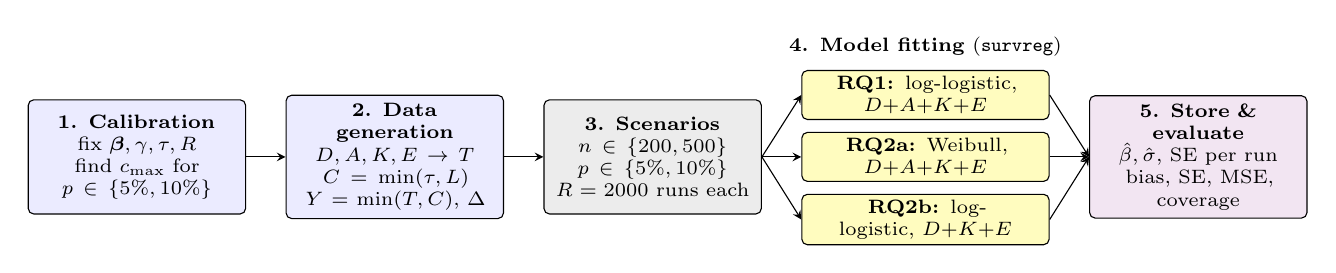
\begin{tikzpicture}[font=\scriptsize,>=stealth,node distance=5mm,
 box/.style={draw,rounded corners=2pt,align=center,inner sep=3pt,text width=2.55cm,minimum height=1.45cm},
 model/.style={draw,rounded corners=2pt,align=center,inner sep=2pt,text width=3.0cm,minimum height=0.5cm,fill=yellow!25}]
\node[box,fill=blue!8] (cal) {\textbf{1. Calibration}\\ fix $\boldsymbol\beta,\gamma,\tau,R$\\ find $c_{\max}$ for\\ $p\in\{5\%,10\%\}$};
\node[box,fill=blue!8,right=of cal] (gen) {\textbf{2. Data generation}\\ $D,A,K,E\to T$\\ $C=\min(\tau,L)$\\ $Y=\min(T,C)$, $\Delta$};
\node[box,fill=gray!15,right=of gen] (sc) {\textbf{3. Scenarios}\\ $n\in\{200,500\}$\\ $p\in\{5\%,10\%\}$\\ $R=2000$ runs each};
\node[model,right=of sc] (m2) {\textbf{RQ2a:} Weibull, $D{+}A{+}K{+}E$};
\node[model,above=1.5mm of m2] (m1) {\textbf{RQ1:} log-logistic, $D{+}A{+}K{+}E$};
\node[model,below=1.5mm of m2] (m3) {\textbf{RQ2b:} log-logistic, $D{+}K{+}E$};
\node[above=0.5mm of m1] {\textbf{4. Model fitting} (\texttt{survreg})};
\node[box,fill=violet!10,right=of m2] (out) {\textbf{5. Store \& evaluate}\\ $\hat\beta,\hat\sigma$, SE per run\\ bias, SE, MSE, coverage};
\draw[->] (cal) -- (gen);
\draw[->] (gen) -- (sc);
\foreach \m in {m1,m2,m3}{\draw[->] (sc.east) -- (\m.west); \draw[->] (\m.east) -- (out.west);}
\end{tikzpicture}
\caption{Simulation workflow: calibration of $c_{\max}$, data generation, the four scenarios, the three model fits and the evaluation.}\label{fig:flow}
\end{figure}
\vspace{-10pt}

\section{Software implementation}
Condensed R code (left: data generation and censoring; right: model fitting and storage).\\[2pt]
\begin{minipage}[t]{0.49\textwidth}
\begin{lstlisting}[style=rcode]
set.seed(123)
beta <- c(b_0 = 5.8, b_d = -0.1, b_a = -0.02,
          b_k = -0.25, b_e = -0.7)
gamma_val <- 1.1; tau <- 90; sim_runs <- 2000
loss_vec <- c(0.05, 0.10)

generate_data <- function(m) {          # covariates
  d <- rgamma(m, shape = 2, scale = 2)
  a <- pmin(pmax(rnorm(m, 45, 15), 18), 85)
  k <- rpois(m, exp(-2.75 + 0.05 * a))
  e <- rbinom(m, 1, plogis(-3.9 + 0.06 * a))
  data.frame(days = d, age = a, nr_comor = k, damage = e)
}
draw_t <- function(x, beta, gamma_val) { # event times
  lambda <- exp(beta["b_0"] + beta["b_d"] * x$days +
    beta["b_a"] * x$age + beta["b_k"] * x$nr_comor +
    beta["b_e"] * x$damage)
  u <- runif(nrow(x))
  lambda * (u / (1 - u))^(1 / gamma_val)
}
# calibrate c_max: P(L < min(T, tau)) = target loss
find_cmax <- function(target, m, cutoff) {
  times <- draw_t(generate_data(m), beta, gamma_val)
  min_t <- pmin(times, cutoff)
  f <- function(cm) mean(pmin(min_t, cm) / cm) - target
  uniroot(f, c(5, max(times)), tol = 0.5)$root
}
cmax <- lapply(loss_vec, find_cmax, m = 1e6, cutoff = tau)

generate_cohort <- function(n, runs, cmax) {
  m <- n * runs                       # all runs at once
  x <- generate_data(m)
  t_event <- draw_t(x, beta, gamma_val)
  cens <- pmin(tau, runif(m, 0, cmax))  # C = min(tau, L)
  data.frame(run_id = rep(seq_len(runs), each = n), x,
             time = pmin(t_event, cens),
             status = as.integer(t_event <= cens))
}
simulated_data <- list(
  n200_loss05 = generate_cohort(200, sim_runs, cmax[[1]]),
  n200_loss10 = generate_cohort(200, sim_runs, cmax[[2]]),
  n500_loss05 = generate_cohort(500, sim_runs, cmax[[1]]),
  n500_loss10 = generate_cohort(500, sim_runs, cmax[[2]]))
saveRDS(simulated_data, "simulated_data.rds")
\end{lstlisting}
\end{minipage}\hfill
\begin{minipage}[t]{0.49\textwidth}
\begin{lstlisting}[style=rcode]
library(survival)
simulated_data <- readRDS("simulated_data.rds")

fit_one_run <- function(d, formula, dist) {
  fit <- tryCatch(survreg(formula, data = d, dist = dist),
                  error = function(e) NULL,
                  warning = function(w) NULL)
  if (is.null(fit)) return(NULL)  # failed / no convergence
  se <- sqrt(diag(vcov(fit)))[names(coef(fit))]
  c(coef(fit), scale = fit$scale,
    setNames(se, paste0("se_", names(se))))
}
fit_model_across_runs <- function(df, formula, dist) {
  est <- lapply(split(df, df$run_id), fit_one_run,
                formula, dist)
  failed <- vapply(est, is.null, logical(1))
  out <- as.data.frame(do.call(rbind, est[!failed]))
  attr(out, "n_failed") <- sum(failed)
  out
}
f_full   <- Surv(time, status) ~ days + age + nr_comor + damage
f_no_age <- Surv(time, status) ~ days + nr_comor + damage
fit_all <- function(f, dist)
  lapply(simulated_data, fit_model_across_runs, f, dist)

model_estimates <- list(
  rq1_loglogistic = fit_all(f_full, "loglogistic"),
  rq2a_weibull    = fit_all(f_full, "weibull"),
  rq2b_no_age     = fit_all(f_no_age, "loglogistic"),
  censoring_rate  = sapply(simulated_data,
                           function(d) 1 - mean(d$status)))
saveRDS(model_estimates, "model_estimates.rds")
\end{lstlisting}
\end{minipage}

\section{Performance measures}
We evaluate the estimates of $\beta_D,\beta_E,\beta_A,\beta_K$, with $\beta_E$ as the main target. In each of the $R=2000$ runs we store the estimate $\hat\beta$ and its standard error. With $\bar\beta$ the average estimate over all runs, we compute:
\textbf{Bias} $=\bar\beta-\beta$: is the estimate systematically wrong?
\textbf{Empirical SE} $=$ the standard deviation of the estimates: how much does the estimate vary between runs? (Variance $=\mathrm{SE}^2$.)
\textbf{MSE} $=$ the average of $(\hat\beta-\beta)^2\approx\mathrm{Bias}^2+\mathrm{Variance}$: the total error.
\textbf{Coverage} $=$ the share of 95\% confidence intervals that contain the true $\beta$: are the standard errors reliable? It should be close to 95\%.
For each scenario we also report the observed censoring rate and the number of runs that failed to converge (these are excluded). Both the log-logistic and the Weibull fits are AFT models fitted with \texttt{survreg}, so their coefficients are on the same scale and can be compared with the same true values. When age is left out, only $\beta_D,\beta_E,\beta_K$ are evaluated.

\section{Alternative (incorrect) analyses}
\textbf{(a) Wrong distribution: fitting a Weibull model.} We fit a Weibull AFT model instead of the log-logistic one. \emph{Why it is wrong:} the Weibull hazard can only increase, decrease or stay constant. It cannot rise and then fall, so it cannot capture the early ``dangerous peak'' in the true hazard.
\textbf{(b) Omitting an important covariate: leaving out age.} We fit the correct log-logistic model, but without age. \emph{Why it is wrong:} age is a confounder. It increases the number of comorbidities ($K$) and the chance of an extra-hepatic cause ($E$), and it also shortens survival directly.

\section{Hypotheses}
\textbf{RQ1: correct log-logistic model.}
\textbf{H1 (bias).} The estimated effects will be very close to the true values in all four scenarios, and any small bias at $n=200$ will be even smaller at $n=500$. The fitted model is the model that generated the data and censoring does not depend on the survival time, so the estimates are correct on average.
\textbf{H2 (sample size).} The empirical SE will drop by about one third and the MSE will fall to roughly 40\% of its value at $n=200$. More patients give more information, and with a bias close to zero the MSE is almost entirely variance.
\textbf{H3 (loss to follow-up).} Going from 5\% to 10\% loss will make the estimates slightly less precise but not biased, an effect much smaller than that of sample size. Extra random censoring only removes some observed events without pushing the estimates in a direction, and many patients are already censored at day 90.

\textbf{RQ2a: Weibull instead of log-logistic.}
\textbf{H4.} The Weibull model will clearly misestimate the intercept and the shape, while the covariate effects will be only slightly biased. The two models differ only in the assumed shape, so most of the misfit is absorbed by the intercept and shape. The Weibull hazard can only go up or down, so it cannot reproduce the early peak; because many patients are censored, the covariate effects will still be somewhat affected.
\textbf{H5.} The Weibull bias will not go away with more patients while its variance will, so it will look relatively worse at $n=500$ than at $n=200$. A wrong model precisely estimates the wrong thing: more data makes the estimate more stable but not more accurate.
\textbf{H6.} The Weibull model will be somewhat more biased at 10\% loss than at 5\%. With more censoring the estimates depend more on the assumed (wrong) shape of the distribution.

\textbf{RQ2b: leaving out the confounder age.}
\textbf{H7.} Comorbidities and damage outside the liver will look more harmful than they really are. In our data older patients have more comorbidities, more often have damage outside the liver and survive shorter, so without age part of its harmful effect is wrongly attributed to $K$ and $E$.
\textbf{H8.} The effect of days to treatment will stay close to its true value but be estimated slightly less precisely. Days to treatment was generated independently of age, so age does not confound it; the survival variation caused by age becomes unexplained noise, which reduces precision but does not push the estimates in a direction.

%=====================================================================
\newpage
\section*{Use of AI tools}
\begin{enumerate}[leftmargin=1.4em,itemsep=3pt]
\item \textbf{Repurposing the censoring calibration function} (05/10/2026; Claude, Anthropic; user: Vrincianu Darius).
\begin{itemize}[leftmargin=1.2em,itemsep=1pt]
\item \textbf{Exact prompt:} ``Help me repurpose the `Calibrate cmax' function from the first assignment for this setup.''
\item \textbf{Summary of output:} Suggested defining an objective function evaluated via \texttt{uniroot} that solves for $c_{\max}$ targeting the loss-to-follow-up probability before $\tau$.
\item \textbf{How it was used:} Implemented as \texttt{find\_cmax} in \texttt{hw2\_simulation.R}.
\item \textbf{Modifications:} Modified and integrated the function based on the suggestion to fit our specific parameter choices and cohort generation pipeline.
\end{itemize}

\item \textbf{Checking code line-by-line and identifying bugs} (07/10/2026; Gemini and Claude via Antigravity; user: Szelestey Adam).
\begin{itemize}[leftmargin=1.2em,itemsep=1pt]
\item \textbf{Exact prompt:} ``Based on the pseudo code in the comments check if my code is correct line-by-line. List if you found any bugs inconsistencies.''
\item \textbf{Summary of output:} Identified that for generating $D$, \texttt{rgamma} should be used instead of \texttt{dgamma}, and noted that standard errors and non-convergence handling were missing after model fitting.
\item \textbf{How it was used:} Corrected the covariate distribution call in \texttt{hw2\_simulation.R} and updated \texttt{fit\_model\_across\_runs} in \texttt{hw2\_model\_fitting.R} to record standard errors and count failed runs.
\item \textbf{Modifications:} Implemented the corrections directly in the simulation scripts.
\end{itemize}

\item \textbf{Flowchart generation} (07/10/2026; Gemini and Claude via Antigravity; user: Szelestey Adam).
\begin{itemize}[leftmargin=1.2em,itemsep=1pt]
\item \textbf{Exact prompt:} ``Based on the provided pseudo code and the code create a compact mermaid flowchart with horizontal layout that fits a single page.''
\item \textbf{Summary of output:} Provided a horizontal flowchart mapping the calibration, data generation, scenarios, model fitting, and evaluation stages.
\item \textbf{How it was used:} Added as Figure~1 in \texttt{draft.md} and transcribed into TikZ for \texttt{main.tex}.
\item \textbf{Modifications:} Replaced mathematical symbols ($Y,\Delta$) with dataset column names (\texttt{time}, \texttt{status}) and condensed stage nodes for readability.
\end{itemize}

\item \textbf{Typesetting the report in LaTeX and page budgeting} (07/10/2026; Gemini and Claude via Antigravity; user: Szelestey Adam).
\begin{itemize}[leftmargin=1.2em,itemsep=1pt]
\item \textbf{Exact prompt:} ``From the markdown document draft.md create a latex report with length of 2 pages that matches the style and format of main.tex (previous report). Make sure to stick to the content one by one. If it doesn't fit the 2 pages give me options where I could cut or compress the content.''
\item \textbf{Summary of output:} A compact 2-page LaTeX draft formatted with two-column code blocks, TikZ flowchart, and concise hypotheses.
\item \textbf{How it was used:} Generated the layout of \texttt{main.tex}.
\item \textbf{Modifications:} Preserved the exact original wording of the research questions, incorporated the group's alternative analysis text, and added the contribution statement and references.
\end{itemize}
\end{enumerate}

\section*{Contribution statement}
\begin{itemize}[leftmargin=1.2em,itemsep=2pt]
\item Avram Andrei: [Hypotheses].
\item Mihaiescu Cristian: [Response to feedback and literature review].
\item Szelestey Adam: [Model fitting programming, compiling the report into LaTeX, flowchart design].
\item Vrincianu Darius: [Data generation and censoring calibration programming].
\item Zeng Qin Tao: [Performance metrics and alternative analysis].
\end{itemize}
All group members confirm that this contribution statement is accurate.

\section*{References}
\begin{itemize}[leftmargin=1.2em,itemsep=2pt]\small
\item Chris-Olaiya, A., Kapoor, A., Ricci, K. S., \& Lindenmeyer, C. C. (2021). Therapeutic plasma exchange in liver failure. \emph{World Journal of Hepatology}, 13(8), 904--915.
\item Huang, D. Q., Terrault, N. A., Tacke, F., et al. (2023). Global epidemiology of cirrhosis --- aetiology, trends and predictions. \emph{Nature Reviews Gastroenterology \& Hepatology}, 20(6), 388--398.
\item Jepsen, P. (2014). Comorbidity in cirrhosis. \emph{World Journal of Gastroenterology}, 20(23), 7223--7230.
\item Larsen, F. S., et al. (2016). High-volume plasma exchange in patients with acute liver failure: An open randomised controlled trial. \emph{Journal of Hepatology}, 64(1), 69--78.
\end{itemize}

\end{document}
